\documentclass{article}
\usepackage{graphicx} % Required for inserting images
\usepackage{graphicx}
\usepackage[letterpaper, portrait, margin=1in]{geometry}
\usepackage{float}
\usepackage{amsmath}
\usepackage{physics}
\usepackage{hyperref}
\usepackage{parskip}
\usepackage{cite}

\title{Doctor, is this normal?\\\large ULAB, Division of Sincerely Serious Science}
\author{Jalen Wong}
\date{\today}

\begin{document}

\maketitle

\section{Introduction}

According to my sources, around May 2021 an image began circulating around the internet about a broken
sidewalk. The image, which can be seen in \autoref{fig:figure1}, claims that the sidewalk crack resembles the form
of a normal distribution. This lab report will test that claim by fitting this curve with a normal standard
distribution (also called a Gaussian distribution).

\begin{figure}[h!]
    \centering
    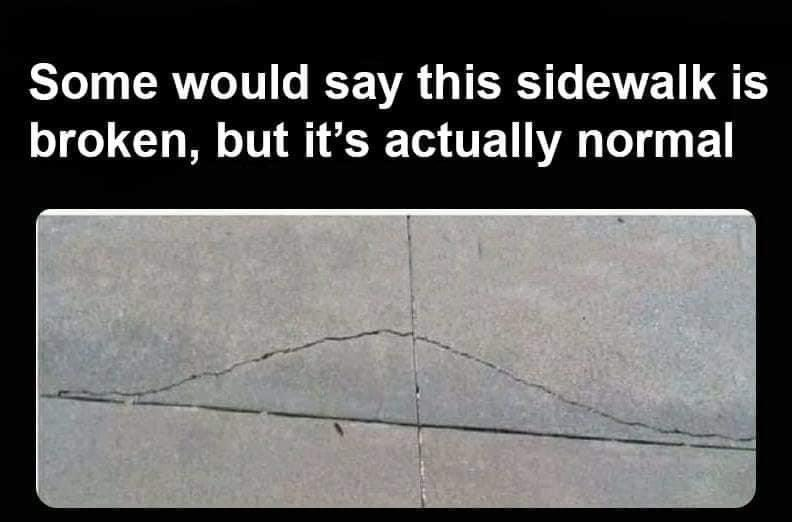
\includegraphics[width=0.8\linewidth]{img.jpg}
    \caption{Sidewalk image from the internet.}
    \label{fig:figure1}
\end{figure}

\section{Methods}
\subsection{Pre-Processing}

First, we used the Perspective Wrap tool in Photoshop to correct the titled perspective of the image. Then,
we worked with the Python Imaging Library and NumPy \cite{2020SciPy-NMeth} and converted our image to grayscale.
A threshold mask was applied to the image so that only dark pixels would be retained. Note that some
minimal manual processing was required to remove the vertical sidewalk crack as well as outlier pixels.
Finally, the location of the dark pixels are recorded as coordinates in a Cartesian plane.

\subsection{Curve Fitting}

We worked with SciPy \cite{2020NumPy-Array} to fit a normal distribution,

\begin{equation}
    f(x) = a \cdot e^{-\frac{1}{2} \frac{(x-\mu)^2}{\sigma}}
\label{eq:curvefit}
\end{equation}

where:
\begin{itemize}
    \item $a$ is a scaling constant,
    \item $\mu$ is the mean, and
    \item $\sigma$ is the standard deviation.
\end{itemize}

\section{Results}

After our data analysis, \autoref{fig:figure2} reveals that a normal distribution fits our data well.

\begin{figure}[h!]
    \centering
    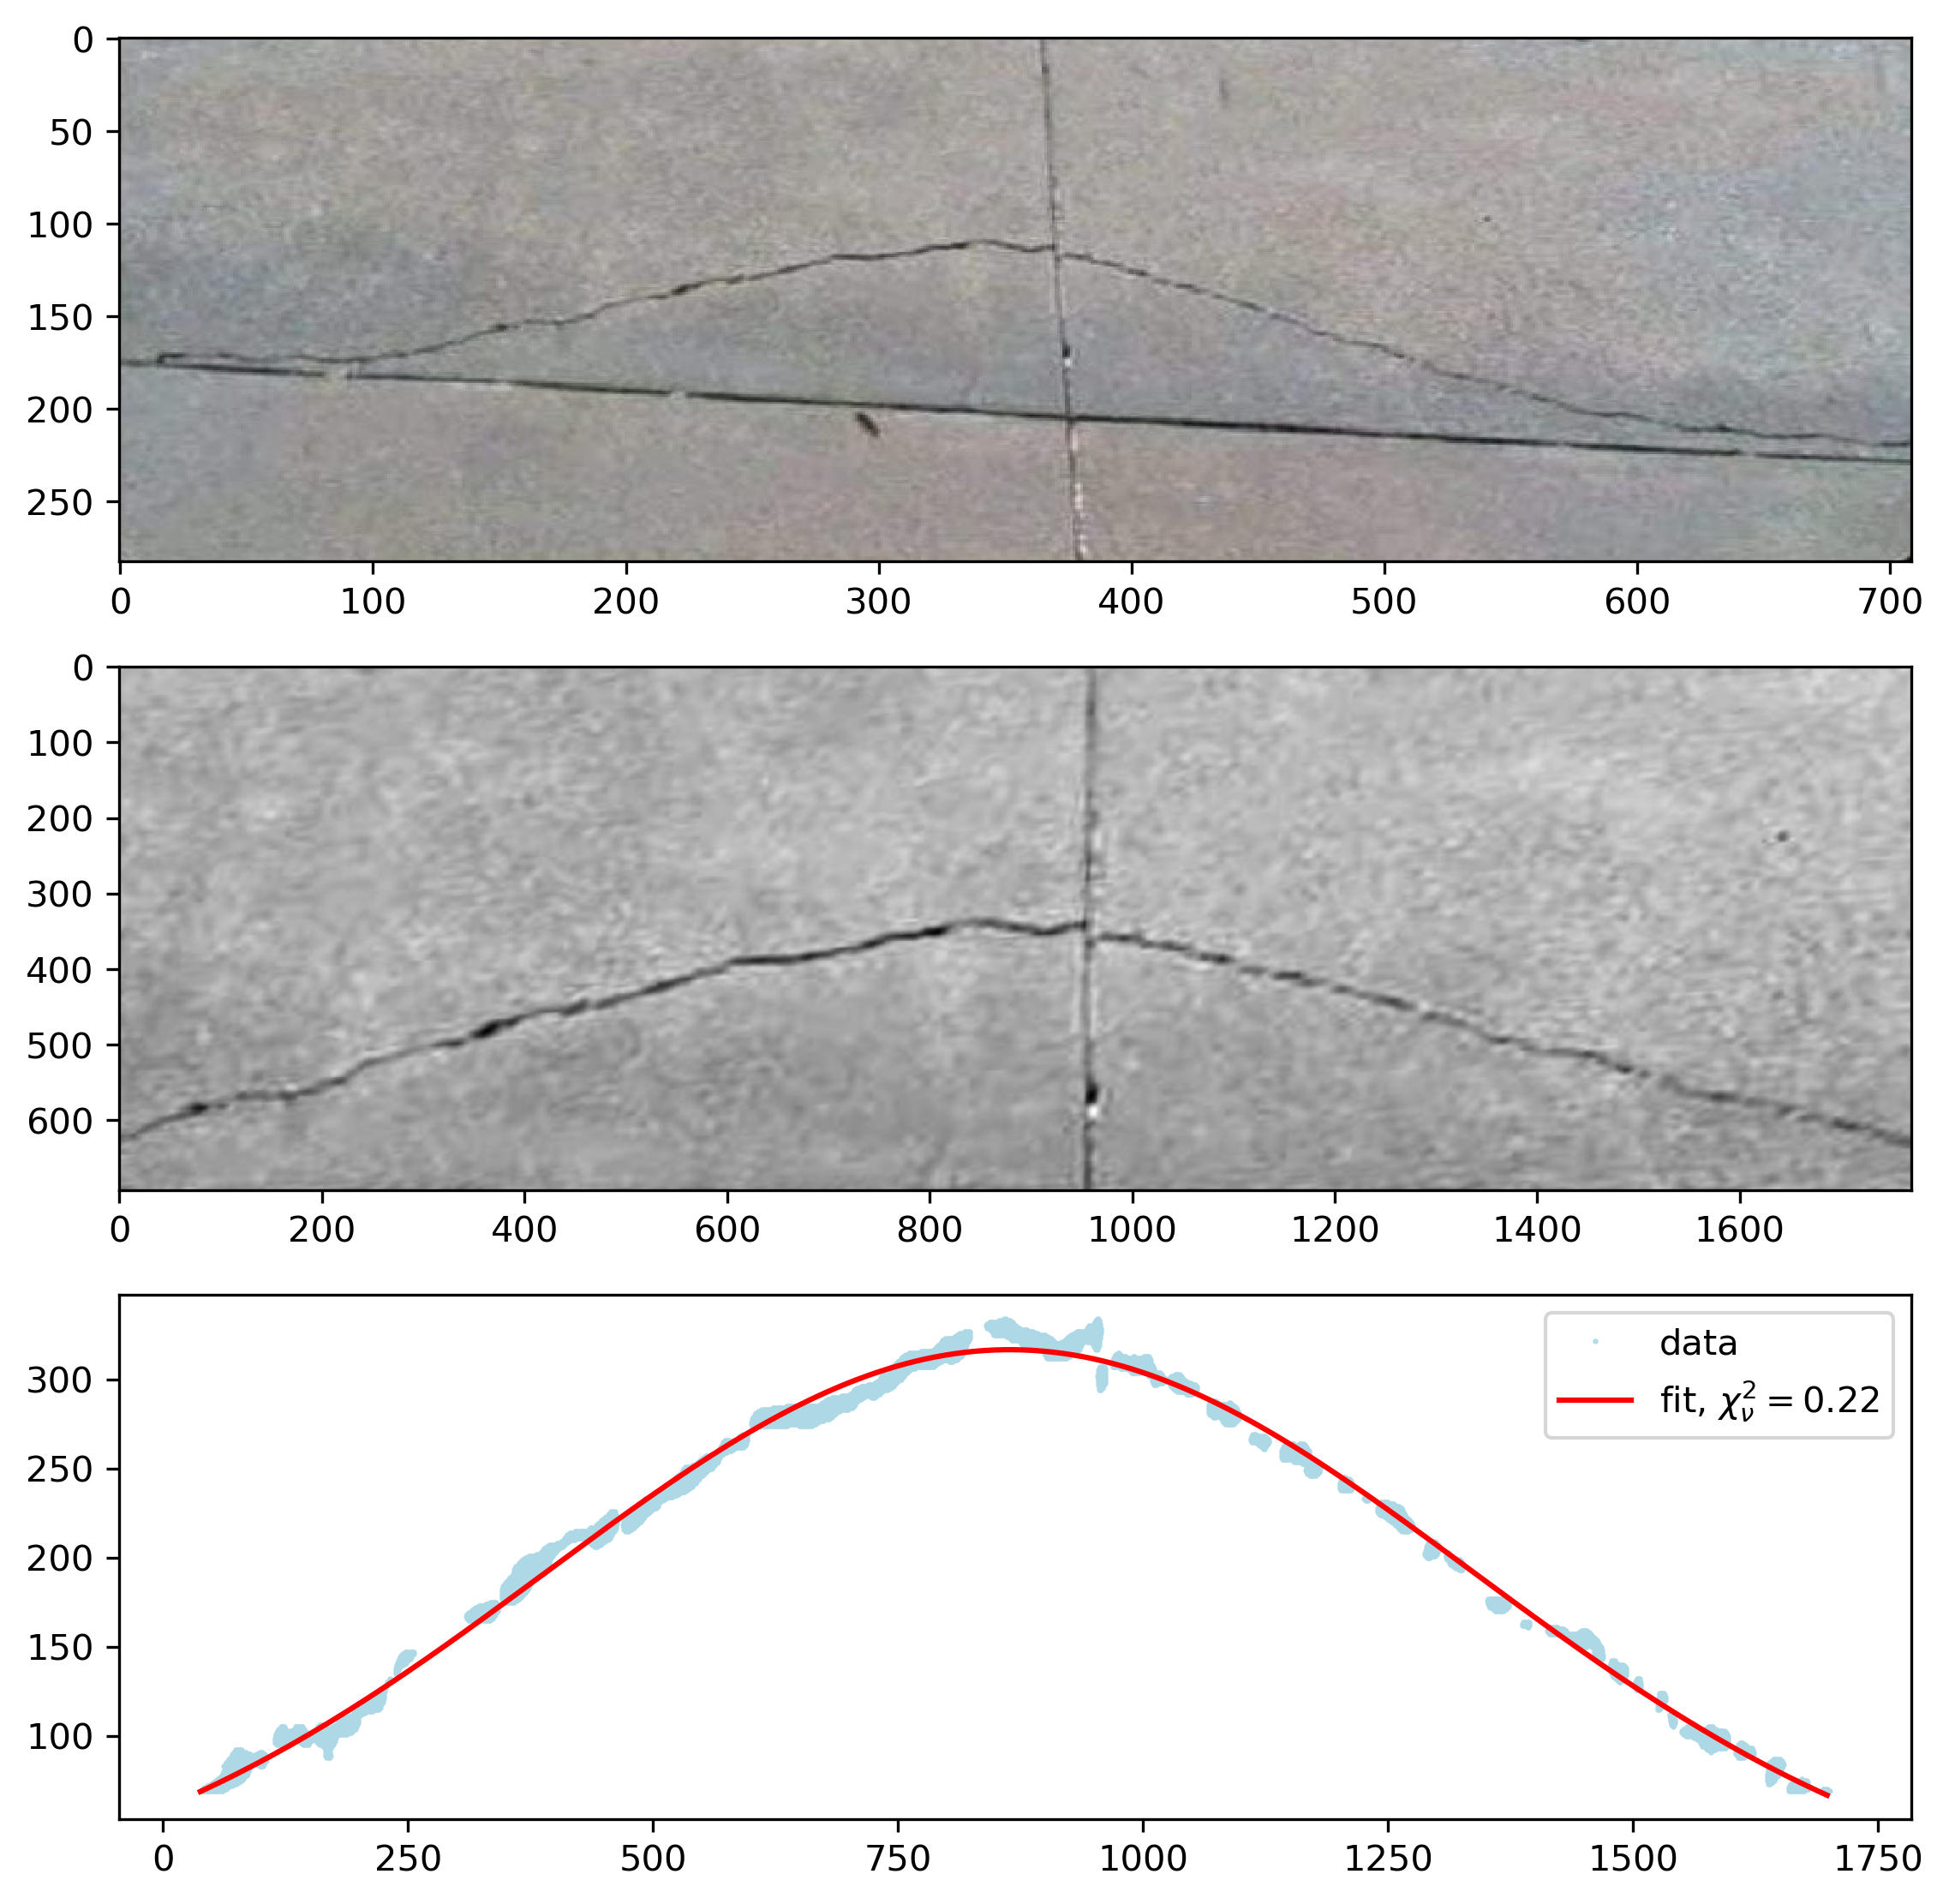
\includegraphics[width=13cm]{fit.png}
    \caption{Top: original image, Middle: processed image with perspective correction and greyscale transformation,
Bottom: curve fit of the sidewalk crack points.}
    \label{fig:figure2}
\end{figure}

Furthermore, we determined the fit to have a reduced chi-squared value:

\begin{equation}
    \chi^2_\nu = \frac{1}{\nu} \sum \frac{(O - E)^2}{E} = 0.22
\label{eq:chisq}
\end{equation}
where $\nu$ is the number of degrees of freedom, $O$ represents the observed values, and $E$ represents the expected values. Of note, we used the Pearson chi-squared definition because it is difficult to estimate the uncertainty of our points.

\bibliographystyle{ieeetr}
\bibliography{ref.bib}
\nocite{*}

\end{document}
